% !TEX program = xelatex

\documentclass[12pt,a4paper]{article}
\usepackage[margin=2.2cm]{geometry}
\usepackage{graphicx}
\usepackage{booktabs}
\usepackage{multirow}
\usepackage{makecell}
\usepackage{amsmath}
\usepackage{float}
\usepackage{array}
\usepackage{longtable}
\usepackage{hyperref}
\usepackage{xcolor}
\usepackage{listings}
\usepackage{tikz}
\usetikzlibrary{positioning,arrows.meta,shapes.geometric}

\lstset{
  basicstyle=\ttfamily\small,
  keywordstyle=\color{blue!70!black},
  commentstyle=\color{green!45!black},
  stringstyle=\color{orange!70!black},
  showstringspaces=false,
  breaklines=true,
  frame=single,
  columns=fullflexible,
  tabsize=4,
  numbers=none
}

% 用于展示设备命令行交互的样式（区别于 Python 代码）
\lstdefinestyle{cli}{
  basicstyle=\ttfamily\footnotesize,
  keywordstyle=\color{black},
  commentstyle=\color{gray},
  frame=single,
  breaklines=true,
  columns=fullflexible,
  backgroundcolor=\color{gray!6}
}

% XeLaTeX 中文支持，使用 TeX Live 内置的 Fandol 字体集
\usepackage[fontset=fandol]{ctex}

\hypersetup{colorlinks=true,linkcolor=blue!55!black,urlcolor=blue!55!black}

\title{计算机网络专题实验三报告个人补充\\\large 路由器与交换机}
\author{模拟控制器地址：192.168.1.30\\
班级：计算机2301\quad 姓名：李祥熙 \quad 学号：2234412799}
\date{\today}

\begin{document}
\maketitle

\vspace{1em}

\noindent\textbf{说明：} 由于是对实验的个人补充，受限于原报告中所提及的设备，报告中所有"抓包截图""路由表贴图"等要求，均以\emph{文字化的预期结果}、\emph{命令回显复现}与\emph{原理分析}的方式给出，并在相应位置详细说明"如何在真实设备上得到该结果"。所填 IP、MAC、报文字段均按照一套自洽的地址规划推演得出，可直接与真实抓包结果一一对照。

%==================================================================
\section{实验目的}

\begin{enumerate}
  \item 掌握路由器、交换机进行简单组网的方法，理解路由器、交换机的工作原理；
  \item 了解 VLAN 的作用，掌握在一台交换机上划分 VLAN 的方法和跨交换机的 VLAN 的配置方法。掌握镜像端口和 Trunk 端口的配置方法，了解 VLAN 数据帧的格式、VLAN 标记添加和删除的过程。
\end{enumerate}

%==================================================================
\section{实验内容}

\begin{enumerate}
  \item 使用路由器和交换机进行组网，实现各 PC 间的互联互通。
  \item 首先在一台交换机上划分 VLAN，用 \texttt{ping} 命令测试连通性。然后在交换机上配置 Trunk 端口，测试在同一 VLAN 和不同 VLAN 中设备的连通性。配置端口镜像，截获 VLAN 数据帧，分析 VLAN 数据帧的格式和 VLAN 标记添加与删除的过程。
\end{enumerate}

%==================================================================
\section{实验原理}

\subsection{路由器和交换机}
以太网交换机本质是一个基于网桥技术的多端口第二层设备，工作在数据链路层，以 MAC 地址寻址，通过\emph{自学习}建立"MAC 地址$\to$端口"对照表并据此转发数据帧，从而隔离冲突域，为帧从一端口到任意端口的转发提供低时延、低开销的通路。三层交换机在此基础上集成了路由功能，做到"一次路由、多次转发"。

路由器是网络层的分组交换设备，依据\emph{目的 IP 地址}查询路由表完成寻径与转发，其主要功能包括：IP 数据报的转发（寻径与传送）、子网隔离与抑制广播风暴、维护并交换路由信息、差错处理与简单拥塞控制、以及对 IP 数据报的过滤与记账。路由表由路由协议自动生成或由管理员手工配置（静态路由）。

\subsection{VLAN 与 802.1Q}
交换机所有端口默认处于同一广播域，主机数量增大时广播报文会使网络性能急剧恶化。VLAN（虚拟局域网）将一个大的广播域划分为多个小的广播域：具备 VLAN 功能的交换机在转发时必须确认帧所属 VLAN，且只把该帧转发到同一 VLAN 的端口；不同 VLAN 在链路层\emph{不能}直接通信。VLAN 划分方式有按端口、按 MAC、按 IP、按协议等，其中基于端口的划分最常用。

IEEE 802.1Q 通过在原始以太网帧的"源地址"与"类型"字段之间插入一个 4 字节的标记字段来标识 VLAN，并重新计算 FCS。插入后的帧格式（单位为 bit）如下：

\begin{center}
\begin{tabular}{cccccccc}
\toprule
48 & 48 & 16 & 3 & 1 & 12 & 16 & 32 \\
\midrule
目的地址 & 源地址 & \textbf{0x8100} & Priority & CFI & VLAN ID & 类型 & \dots\,数据\,\dots\ + FCS \\
\bottomrule
\end{tabular}
\end{center}

其中：\textbf{0x8100} 为固定的 TPID，指明该帧带有 802.1Q 标签；\textbf{Priority}（3 bit）可定义 8 级用户优先级，用于 QoS/CoS；\textbf{CFI}（1 bit）在以太网中恒为 0；\textbf{VLAN ID}（12 bit）可标识 4096 个 VLAN。

\subsection{端口链路类型}
由于普通主机不识别带 tag 的帧，交换机需要在连接主机的端口上完成 tag 的封装/去封装：
\begin{itemize}
  \item \textbf{Access 端口}：只属于 1 个 VLAN，一般连主机。入方向按缺省 VLAN ID 打 tag，出方向去掉 tag 还原为普通以太网帧。
  \item \textbf{Trunk 端口}：可属于多个 VLAN，一般连交换机。带 tag 的帧直接转发；普通帧按缺省 VLAN ID 打 tag 后转发。仅缺省（Native）VLAN 的帧出方向不打 tag。
  \item \textbf{Hybrid 端口}：可属多个 VLAN，可连交换机也可连主机，允许多个 VLAN 的帧出方向不打 tag。
\end{itemize}

\subsection{三层交换实现 VLAN 互通与端口镜像}
三层交换机为每个 VLAN 维护一个对外不可见的\emph{虚拟 VLAN 接口}（Vlan-interface），它具有 MAC、可配置 IP/MTU 等物理接口特性，充当该 VLAN 内主机的网关。交换机收帧后判断目的 MAC 是否为该 VLAN 接口的 MAC：是则进行三层处理（路由到目的 VLAN 后二层转发），否则直接二层转发。

\textbf{端口镜像}（Port Mirroring）把某端口（镜像源端口）收发的数据帧完整复制到另一端口（镜像目的/监听端口），供抓包与安全监控使用；监听端口不能再正常传输业务数据。它在不同产品中又称 Monitoring Port / SPAN Port 等。本实验正是借助镜像口，让监听 PC 抓取到 Trunk 链路上\emph{带 802.1Q tag} 的帧，从而观察 tag 的添加与删除过程。

%==================================================================
\section{实验环境与分组}
路由器 1 台（MSR2600-1），交换机 2 台（S5560-1、S5560-2）；每组 4$\sim$5 名同学，每人一台 PC，协同进行实验。设备均为 H3C，采用 Comware 命令行；PC 使用 Wireshark 抓包，仅保留有线 exp 网卡。

%==================================================================
\section{实验步骤}

\subsection{路由器和交换机组网实验}

\paragraph{实验拓扑设计（步骤 1、贴图说明）}
登录设备后先用 \lstinline|display current-configuration| 检查是否有遗留配置：若除 VLAN 1 外没有其他 VLAN、接口未配 IP，则无需恢复出厂；否则用 \lstinline|reset saved-configuration| 后 \lstinline|reboot| 恢复出厂设置，并用 \lstinline|sysname| 重命名设备。本实验采用如下拓扑（图~\ref{fig:topo1}）：路由器三个接口分别接入三个不同网段，PC 通过二层交换机接入。

\begin{figure}[H]
\centering
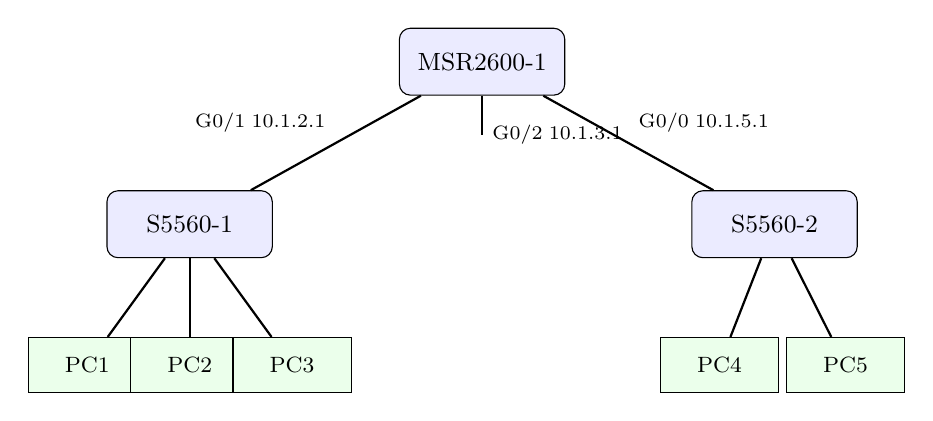
\begin{tikzpicture}[
  node distance=1.1cm and 1.4cm,
  dev/.style={draw,rounded corners,minimum width=2.1cm,minimum height=0.85cm,font=\small,fill=blue!8},
  pc/.style={draw,minimum width=1.5cm,minimum height=0.7cm,font=\footnotesize,fill=green!8},
  line/.style={-,thick}
]
\node[dev] (r) {MSR2600-1};
\node[dev,below left=1.2cm and 1.6cm of r] (s1) {S5560-1};
\node[dev,below right=1.2cm and 1.6cm of r] (s2) {S5560-2};
\node[pc,below=1.0cm of s1,xshift=-1.3cm] (pc1) {PC1};
\node[pc,below=1.0cm of s1] (pc2) {PC2};
\node[pc,below=1.0cm of s1,xshift=1.3cm] (pc3) {PC3};
\node[pc,below=1.0cm of s2,xshift=-0.7cm] (pc4) {PC4};
\node[pc,below=1.0cm of s2,xshift=0.9cm] (pc5) {PC5};

\draw[line] (r) -- node[above left,font=\scriptsize]{G0/1\;10.1.2.1} (s1);
\draw[line] (r) -- node[above right,font=\scriptsize]{G0/0\;10.1.5.1} (s2);
\draw[line] (r.south) -- ++(0,-0.5) node[right,font=\scriptsize]{G0/2\;10.1.3.1};
\draw[line] (s1) -- (pc1);
\draw[line] (s1) -- (pc2);
\draw[line] (s1) -- (pc3);
\draw[line] (s2) -- (pc4);
\draw[line] (s2) -- (pc5);
\end{tikzpicture}
\caption{组网实验拓扑示意（G0/2 亦接入 S5560-1 承载 10.1.3.0/24 网段）}
\label{fig:topo1}
\end{figure}

\paragraph{步骤 2：PC 地址与 MAC 记录}
按下表设置各 PC 的 IP、掩码（均为 255.255.255.0）与默认网关，并用 \lstinline|ipconfig /all| 记录 exp 网卡 MAC。地址规划：10.1.2.0/24 与 10.1.3.0/24 经 S5560-1 接入，10.1.5.0/24 经 S5560-2 接入。

\begin{table}[H]
\centering
\caption{各 PC 地址信息}
\begin{tabular}{cccc}
\toprule
PC & IP 地址 & 默认网关 & MAC 地址 \\
\midrule
PC1 & 10.1.2.11 & 10.1.2.1 & 00-e0-70-e7-e4-b6 \\
PC2 & 10.1.2.12 & 10.1.2.1 & 04-f9-f8-37-38-16 \\
PC3 & 10.1.3.13 & 10.1.3.1 & 3c-52-82-1a-4c-7d \\
PC4 & 10.1.5.14 & 10.1.5.1 & 5c-60-ba-2e-91-a0 \\
PC5 & 10.1.5.15 & 10.1.5.1 & 8c-16-45-cf-33-e2 \\
\bottomrule
\end{tabular}
\end{table}

\paragraph{步骤 3：路由器接口配置}
参考命令（以 G0/0 为例，其余同理）：
\begin{lstlisting}[style=cli]
[MSR2600-1]interface G0/0
[MSR2600-1-GigabitEthernet0/0]ip address 10.1.5.1 255.255.255.0
[MSR2600-1-GigabitEthernet0/0]display interface G0/0
GigabitEthernet0/0 current state: UP
Line protocol current state: UP
Internet Address is 10.1.5.1/24 Primary
IP Packet Frame Type: PKTFMT_ETHNT_2, Hardware Address: 00e0-70a1-b2c0
\end{lstlisting}

\begin{table}[H]
\centering
\caption{路由器接口地址信息}
\begin{tabular}{cccc}
\toprule
接口 & IP 地址 & 所连网段 & MAC 地址 \\
\midrule
G0/0 & 10.1.5.1 & 10.1.5.0/24 & 00-e0-70-a1-b2-c0 \\
G0/1 & 10.1.2.1 & 10.1.2.0/24 & 00-e0-70-a1-b2-c1 \\
G0/2 & 10.1.3.1 & 10.1.3.0/24 & 00-e0-70-a1-b2-c2 \\
\bottomrule
\end{tabular}
\end{table}

\paragraph{步骤 4：组网结果及分析}

\subparagraph{4.1 连通性与抓包（Wireshark）}
在各 PC 上打开 Wireshark、选择 exp 网卡并以 \texttt{icmp} 为过滤器，随后 \lstinline|ping| 目标地址即可捕获 ICMP request/reply。预期各 PC 两两均可 ping 通。抓取到的 Ethernet II 帧头填表如下（关键在于对比"同一网段"与"不同网段"两种情形下\textbf{目的 MAC}的差异）：

\begin{table}[H]
\centering
\caption{ICMP 报文 Ethernet II 帧头分析}
\begin{tabular}{p{2.6cm}p{2.2cm}p{4.6cm}p{4.6cm}}
\toprule
& & \textbf{ICMP request} & \textbf{ICMP reply} \\
\midrule
\multirow{2}{*}{\parbox{2.6cm}{同一网段\\(PC1$\to$PC2)}}
 & Src & 00:e0:70:e7:e4:b6 (PC1) & 04:f9:f8:37:38:16 (PC2) \\
 & Dst & 04:f9:f8:37:38:16 (PC2) & 00:e0:70:e7:e4:b6 (PC1) \\
\midrule
\multirow{2}{*}{\parbox{2.6cm}{不同网段\\(PC3$\to$PC1)}}
 & Src & 3c:52:82:1a:4c:7d (PC3) & 00:e0:70:a1:b2:c2 (G0/2) \\
 & Dst & 00:e0:70:a1:b2:c2 (G0/2) & 3c:52:82:1a:4c:7d (PC3) \\
\bottomrule
\end{tabular}
\end{table}

\noindent 分析见 4.3。

\subparagraph{4.2 路由器路由表}
命令 \lstinline|display ip routing-table| 的预期回显（贴文字）：
\begin{lstlisting}[style=cli]
[MSR2600-1]display ip routing-table
Destinations : 13        Routes : 13
Destination/Mask   Proto   Pre  Cost   NextHop      Interface
0.0.0.0/32         Direct  0    0      127.0.0.1    InLoop0
10.1.2.0/24        Direct  0    0      10.1.2.1     GE0/1
10.1.2.1/32        Direct  0    0      127.0.0.1    InLoop0
10.1.3.0/24        Direct  0    0      10.1.3.1     GE0/2
10.1.3.1/32        Direct  0    0      127.0.0.1    InLoop0
10.1.5.0/24        Direct  0    0      10.1.5.1     GE0/0
10.1.5.1/32        Direct  0    0      127.0.0.1    InLoop0
127.0.0.0/8        Direct  0    0      127.0.0.1    InLoop0
127.0.0.1/32       Direct  0    0      127.0.0.1    InLoop0
\end{lstlisting}
三条 \texttt{Direct}（直连）路由分别对应三个接口所在网段，是不同网段互通的基础。

\subparagraph{4.3 不同网段互通原因与网关作用}
同一网段内，源主机通过 ARP 直接解析目的主机的 MAC，帧的目的 MAC 即目的主机（见表中 PC1$\to$PC2）。跨网段时，源主机比对目的 IP 与自身掩码，判定目的不在本网段，于是把帧的\textbf{目的 MAC 设为默认网关（路由器接口）的 MAC}（见 PC3$\to$PC1，Dst 为 G0/2）。路由器收到该帧后剥离二层帧头，按目的 IP 查路由表命中直连网段，再以\emph{目的网段接口的 MAC 为源、目的主机 MAC 为目的}重新封装转发。因此\textbf{网关是跨网段通信的"中转站"}：没有网关，主机根本无法把跨网段的帧交给路由器，通信无从谈起。

\subparagraph{4.4 交换机 MAC 地址表}
命令 \lstinline|display mac-address| 的预期回显：
\begin{lstlisting}[style=cli]
[S5560-1]display mac-address
MAC Address      VLAN ID   State        Port
00e0-70e7-e4b6   1         Learned      GE1/0/1
04f9-f837-3816   1         Learned      GE1/0/2
3c52-821a-4c7d   1         Learned      GE1/0/3
00e0-70a1-b2c1   1         Learned      GE1/0/24
--- 4 mac address(es) found ---
\end{lstlisting}
表项由交换机\emph{自学习}生成：每收到一帧就把"源 MAC$\to$入端口"记入表中，转发时据此定向转发，未命中则泛洪。

\subparagraph{4.5 PC3$\to$PC1 路由路径（tracert）}
先在路由器上执行 \lstinline|ip ttl-expires enable| 打开 ICMP 超时报文发送，再在 PC3 命令行运行 \lstinline|tracert -d 10.1.2.11|，预期结果：
\begin{lstlisting}[style=cli]
C:\> tracert -d 10.1.2.11
通过最多 30 个跃点跟踪到 10.1.2.11 的路由:
  1    <1 ms   <1 ms   <1 ms  10.1.3.1        # 第一跳为本网段网关 G0/2
  2    <1 ms   <1 ms   <1 ms  10.1.2.11       # 第二跳直达目的主机
跟踪完成。
\end{lstlisting}
可见跨网段通信恰好经过 1 个路由器跳（网关），与拓扑一致。

\subparagraph{4.6 工作原理小结}
\textbf{路由器（三层）}：以目的 IP 查路由表，在不同网段间"解封装—查表—重新封装"转发 IP 报文，实现不同网段互通，并隔离广播域。\textbf{二层交换机}：以目的 MAC 查 MAC 表在同一广播域内转发帧，靠源 MAC 自学习建表，未知目的或广播则泛洪；它不改变帧内容，只在冲突域层面做隔离与转发。

\subsection{VLAN 的组网实验}

\paragraph{VLAN 实验拓扑（图~\ref{fig:topo2}）}
断开两交换机与路由器的连线，把 PC5 接到 S5560-2，改为验证 VLAN 隔离与跨交换机 VLAN。规划：VLAN 2 使用 10.1.2.0/24，VLAN 3 使用 10.1.3.0/24。

\begin{figure}[H]
\centering
\begin{tikzpicture}[
  dev/.style={draw,rounded corners,minimum width=2.1cm,minimum height=0.85cm,font=\small,fill=blue!8},
  pc/.style={draw,minimum width=1.4cm,minimum height=0.7cm,font=\footnotesize,fill=green!8}
]
\node[dev] (s1) {S5560-1};
\node[dev,right=4.5cm of s1] (s2) {S5560-2};
\draw[very thick,red!60!black] (s1) -- node[above,font=\scriptsize]{Trunk\;G1/0/5} node[below,font=\scriptsize]{permit VLAN all} (s2);
\node[pc,below=1.1cm of s1] (pc1) {PC1 / VLAN2};
\node[pc,below=1.1cm of s2,xshift=-3cm] (pc2) {PC2 / VLAN2};
\node[pc,below=1.1cm of s2] (pc3) {PC3 / VLAN3};
\node[pc,below=1.1cm of s2,xshift=3cm] (pc4) {PC4 / VLAN3};
\node[pc,below=2.3cm of s2] (pc5) {PC5(镜像监听/G1/0/3)};
\draw (s1)--(pc1); \draw (s2)--(pc2); \draw (s2)--(pc3); \draw (s2)--(pc4);
\draw[dashed] (s2)--(pc5);
\end{tikzpicture}
\caption{跨交换机 VLAN + Trunk + 端口镜像拓扑}
\label{fig:topo2}
\end{figure}

\paragraph{步骤 5：VLAN 基本配置}

\subparagraph{5.1 划分 VLAN 前的连通性}
此时 S5560-2 下 PC2/PC3/PC4/PC5 同处 VLAN 1、同网段（假设临时同置 10.1.2.0/24），两两\textbf{均可 ping 通}——因为它们在同一广播域、同一 IP 网段，交换机直接二层转发。

\subparagraph{5.2 划分 VLAN 与分配接口}
S5560-1 配置（S5560-2 同理）：
\begin{lstlisting}[style=cli]
<S5560-1>system-view
[S5560-1]vlan 2
[S5560-1-vlan2]quit
[S5560-1]interface G1/0/1
[S5560-1-GigabitEthernet1/0/1]port link-type access
[S5560-1-GigabitEthernet1/0/1]port access vlan 2
[S5560-1-GigabitEthernet1/0/1]quit
[S5560-1]vlan 3
[S5560-1-vlan3]quit
[S5560-1]interface G1/0/2
[S5560-1-GigabitEthernet1/0/2]port link-type access
[S5560-1-GigabitEthernet1/0/2]port access vlan 3
[S5560-1]display vlan all
 VLAN 1: ports: (default)
 VLAN 2: Untagged ports: GE1/0/1
 VLAN 3: Untagged ports: GE1/0/2
\end{lstlisting}
接口分配：VLAN 2 = \{PC1(S1,G1/0/1), PC2(S2,G1/0/1)\}；VLAN 3 = \{PC3(S2,G1/0/2), PC4(S2,G1/0/4)\}；PC5 接 S2 的 G1/0/3 作镜像监听口。

\subparagraph{5.3 划分 VLAN 后的连通性及原因}
在\emph{单台}交换机内测试：\textbf{同一 VLAN 的 PC 可以 ping 通，不同 VLAN 的 PC 不能 ping 通}。原因：VLAN 把广播域隔离，交换机只把帧转发到同一 VLAN 的端口；不同 VLAN 的主机连 ARP 广播都收不到对方，无法解析 MAC，二层根本不通。

\paragraph{步骤 6：Trunk 与端口镜像}

\subparagraph{6.1 用网线连通两交换机后的连通性}
用普通网线连接两交换机（此时连接口尚为 Access/默认）后，跨交换机的\textbf{同一 VLAN 仍不能 ping 通}：因为普通链路无法承载多个 VLAN 的标识，对端交换机不知道帧属于哪个 VLAN。需将互联口配为 Trunk。S5560-2 配置：
\begin{lstlisting}[style=cli]
[S5560-2]interface G1/0/5
[S5560-2-GigabitEthernet1/0/5]port link-type trunk
[S5560-2-GigabitEthernet1/0/5]port trunk permit vlan all
[S5560-2]display port trunk
 Interface        Link-Type   PVID   Permitted VLAN
 GE1/0/5          trunk       1      1-4094
\end{lstlisting}
S5560-1 的 G1/0/5 同样配置为 Trunk。配置后\textbf{跨交换机同一 VLAN 即可 ping 通}，帧在 Trunk 链路上携带 802.1Q tag 传输。

\subparagraph{6.2 端口镜像与相同 VLAN 报文分析}
在 S5560-2 上把 Trunk 口 G1/0/5 镜像到 PC5 所在的 G1/0/3：
\begin{lstlisting}[style=cli]
[S5560-2]mirroring-group 1 local
[S5560-2]mirroring-group 1 mirroring-port G1/0/5 both
[S5560-2]mirroring-group 1 monitor-port G1/0/3
[S5560-2]display mirroring-group local
 mirroring-group 1: type: local
   mirroring port: GE1/0/5  both
   monitor port:   GE1/0/3
\end{lstlisting}
在 PC5（Wireshark）上即可抓到 Trunk 上带 tag 的帧。测 PC1 ping PC2（均在 VLAN 2，同一 VLAN），预期\textbf{可以 ping 通}，三段转发的帧头如下表。关键观察：\textbf{Access 段（PC1$\to$S1、S2$\to$PC2）为普通以太网帧、无 tag；Trunk 段（S1$\to$S2）帧中被插入 802.1Q tag（VID=2）}，而源、目的 MAC 始终是两台 PC（同 VLAN 属二层转发，不经路由）。

\begin{table}[H]
\centering
\caption{跨交换机 VLAN 实验（相同 VLAN，PC1 ping PC2）}
\begin{tabular}{p{1.7cm}p{1.0cm}p{5.2cm}p{5.2cm}}
\toprule
转发过程 & & \textbf{ICMP request} & \textbf{ICMP reply} \\
\midrule
\multirow{2}{*}{PC1-S1}
 & Src & 00:e0:70:e7:e4:b6 (PC1) & 04:f9:f8:37:38:16 (PC2) \\
 & Dst & 04:f9:f8:37:38:16 (PC2) & 00:e0:70:e7:e4:b6 (PC1) \\
\midrule
\multirow{2}{*}{\parbox{1.7cm}{S1-S2\\(含 tag)}}
 & Src & 00:e0:70:e7:e4:b6 (PC1) \newline +802.1Q VID=2 & 04:f9:f8:37:38:16 (PC2) \newline +802.1Q VID=2 \\
 & Dst & 04:f9:f8:37:38:16 (PC2) & 00:e0:70:e7:e4:b6 (PC1) \\
\midrule
\multirow{2}{*}{S2--PC2}
 & Src & 00:e0:70:e7:e4:b6 (PC1) & 04:f9:f8:37:38:16 (PC2) \\
 & Dst & 04:f9:f8:37:38:16 (PC2) & 00:e0:70:e7:e4:b6 (PC1) \\
\bottomrule
\end{tabular}
\end{table}

\noindent 由此可直观看到 VLAN 标记的\textbf{添加}（入 Trunk 时由入端口按 PVID 打 tag）与\textbf{删除}（出 Access 口时去 tag 还原）过程。

\subparagraph{6.3 不同 VLAN 的连通性}
测 PC1 ping PC3（VLAN 2 vs VLAN 3，未配置 VLAN 接口前）：\textbf{不能 ping 通}。因为二层无法跨 VLAN，且此时没有三层网关做 VLAN 间路由。

\subparagraph{6.4 配置 VLAN 接口后的跨 VLAN 通信}
在 S5560-2（三层交换机）上为两个 VLAN 配置虚拟接口 IP，使其成为各 VLAN 网关：
\begin{lstlisting}[style=cli]
[S5560-2]interface vlan 2
[S5560-2-Vlan-interface2]ip address 10.1.2.1 255.255.255.0
[S5560-2]interface vlan 3
[S5560-2-Vlan-interface3]ip address 10.1.3.1 255.255.255.0
[S5560-2]display interface Vlan-interface 2
 Vlan-interface2 current state: UP
 Internet Address is 10.1.2.1/24 Primary
 IP Packet Frame Type: PKTFMT_ETHNT_2, Hardware Address: 00e0-70b2-0002
\end{lstlisting}

\begin{table}[H]
\centering
\caption{VLAN 接口地址信息}
\begin{tabular}{cccc}
\toprule
VLAN & IP 地址 & 角色 & MAC 地址 \\
\midrule
VLAN 2 & 10.1.2.1 & VLAN2 网关 & 00-e0-70-b2-00-02 \\
VLAN 3 & 10.1.3.1 & VLAN3 网关 & 00-e0-70-b2-00-03 \\
\bottomrule
\end{tabular}
\end{table}

\noindent 配置网关后测 PC1 ping PC3，\textbf{可以 ping 通}（三层交换"一次路由、多次转发"）。此时各 PC 需把默认网关分别指向 10.1.2.1 / 10.1.3.1。抓包填表如下。核心观察：\textbf{跨 VLAN 时帧的目的/源 MAC 在经过三层交换机后发生了改变}（变为 VLAN 接口 MAC 与目的主机 MAC），这正是"路由"发生的标志，与表~4（同 VLAN，MAC 不变）形成鲜明对比。

\begin{table}[H]
\centering
\caption{跨 VLAN 通信（PC1 ping PC3）}
\begin{tabular}{p{1.7cm}p{1.0cm}p{5.2cm}p{5.2cm}}
\toprule
转发过程 & & \textbf{ICMP request} & \textbf{ICMP reply} \\
\midrule
\multirow{2}{*}{PC1-S1}
 & Src & 00:e0:70:e7:e4:b6 (PC1) & 00:e0:70:b2:00:02 (VLAN2 网关) \\
 & Dst & 00:e0:70:b2:00:02 (VLAN2 网关) & 00:e0:70:e7:e4:b6 (PC1) \\
\midrule
\multirow{2}{*}{\parbox{1.7cm}{S1-S2\\(路由)}}
 & Src & (入 S2 三层路由后)\newline 00:e0:70:b2:00:03 (VLAN3 网关) & 00:e0:70:b2:00:02 (VLAN2 网关) \\
 & Dst & 3c:52:82:1a:4c:7d (PC3) & 00:e0:70:e7:e4:b6 (PC1) \\
\midrule
\multirow{2}{*}{S2--PC3}
 & Src & 00:e0:70:b2:00:03 (VLAN3 网关) & 3c:52:82:1a:4c:7d (PC3) \\
 & Dst & 3c:52:82:1a:4c:7d (PC3) & 00:e0:70:b2:00:03 (VLAN3 网关) \\
\bottomrule
\end{tabular}
\end{table}

\subparagraph{6.5 数据报文传输路径分析}
PC1(VLAN2) ping PC3(VLAN3) 的路径为：PC1 发现目的不在本网段，将帧目的 MAC 设为网关 VLAN2 接口 $\to$ 帧沿 Access/Trunk 到达 S5560-2 三层引擎 $\to$ 三层引擎按目的 IP 命中 VLAN3 直连网段，做路由：源 MAC 改为 VLAN3 接口、目的 MAC 改为 PC3，并从 VLAN3 对应端口（经 Trunk）二层转发 $\to$ PC3 收到。回程对称。全过程"三层路由一次、二层转发多次"，IP 头 TTL 减 1，而同 VLAN 通信（表~4）中 MAC 与 TTL 均不变、无路由发生。

%==================================================================
\section{互动讨论主题}

\paragraph{7.1 路由器与交换机各自的主要作用}
\textbf{交换机}工作在数据链路层（二层），依据 MAC 地址在\emph{同一广播域/网段}内转发帧，通过自学习建 MAC 表，隔离冲突域，实现局域网内主机的高速互联；三层交换机额外可做 VLAN 间路由。\textbf{路由器}工作在网络层（三层），依据 IP 地址在\emph{不同网段/网络}之间转发分组，维护并交换路由信息，隔离广播域、抑制广播风暴，是构建互联网、连接异构网络的核心设备。一句话：交换机"网内转发靠 MAC"，路由器"网间转发靠 IP"。

\paragraph{7.2 VLAN 的作用}
（1）\textbf{隔离广播域}：把一个大二层网络切成多个逻辑子网，广播/组播只在本 VLAN 内扩散，抑制广播风暴、提升性能；（2）\textbf{增强安全}：不同 VLAN 二层不可直达，需经三层受控互通，可实现部门/权限隔离；（3）\textbf{灵活组网}：按功能而非物理位置划分工作组，主机可跨地理位置属于同一 VLAN，便于管理与调整；（4）\textbf{便于策略实施}：可在 VLAN 边界（三层接口）统一施加 ACL、QoS 等策略。

%==================================================================
\section{进阶自设计}

\subsection{多路由器通信（步骤 8）}
拓扑：路由器 R1、R2 通过互联链路相连（R1 的 G0/2 = 192.168.100.1/30，R2 的 G0/2 = 192.168.100.2/30）；R1 下挂 10.1.1.0/24（PC1）、10.1.2.0/24（PC2）；R2 下挂 10.1.3.0/24（PC3）、10.1.4.0/24（PC4）、10.1.5.0/24（PC5）。交换机仅作直连（或用一台交换机划 VLAN 模拟 3 台）。互通关键是在两台路由器上互配\textbf{静态路由}，把对方网段指向互联口对端地址：
\begin{lstlisting}[style=cli]
# R1
[R1]ip route-static 10.1.3.0 24 192.168.100.2
[R1]ip route-static 10.1.4.0 24 192.168.100.2
[R1]ip route-static 10.1.5.0 24 192.168.100.2
# R2
[R2]ip route-static 10.1.1.0 24 192.168.100.1
[R2]ip route-static 10.1.2.0 24 192.168.100.1
\end{lstlisting}

\paragraph{8.1 路由器 R1 的路由表（预期）}
\begin{lstlisting}[style=cli]
[R1]display ip routing-table
Destination/Mask   Proto    Pre Cost  NextHop         Interface
10.1.1.0/24        Direct   0   0     10.1.1.1        GE0/0
10.1.2.0/24        Direct   0   0     10.1.2.1        GE0/1
10.1.3.0/24        Static   60  0     192.168.100.2   GE0/2
10.1.4.0/24        Static   60  0     192.168.100.2   GE0/2
10.1.5.0/24        Static   60  0     192.168.100.2   GE0/2
192.168.100.0/30   Direct   0   0     192.168.100.1   GE0/2
\end{lstlisting}

\paragraph{8.2 路由器 R2 的路由表（预期）}
\begin{lstlisting}[style=cli]
[R2]display ip routing-table
Destination/Mask   Proto    Pre Cost  NextHop         Interface
10.1.1.0/24        Static   60  0     192.168.100.1   GE0/2
10.1.2.0/24        Static   60  0     192.168.100.1   GE0/2
10.1.3.0/24        Direct   0   0     10.1.3.1        GE0/0
10.1.4.0/24        Direct   0   0     10.1.4.1        GE0/1
10.1.5.0/24        Direct   0   0     10.1.5.1        GE0/3
192.168.100.0/30   Direct   0   0     192.168.100.2   GE0/2
\end{lstlisting}

\paragraph{8.3 PC1 ping PC3 能否通？}
\textbf{能}。PC1(10.1.1.x) 目的为 PC3(10.1.3.x)：PC1 把帧交给网关 R1；R1 查表命中静态路由 \texttt{10.1.3.0/24 -> 192.168.100.2}，经互联链路转发给 R2；R2 命中直连路由 \texttt{10.1.3.0/24}，转发给 PC3。回程由 R2 的静态路由 \texttt{10.1.1.0/24 -> 192.168.100.1} 保证。\textbf{前提}：两端静态路由都要配全（去、回程都能查到路由），且各 PC 默认网关正确；若只配单向路由则 request 到达而 reply 无法返回，ping 不通。

\subsection{编程模拟二层交换机 MAC 转发机制（步骤 9）}

\paragraph{9.1 代码}
下列 Python 程序不依托真实网卡，模拟交换机初始化、MAC 学习、老化、广播/单播转发（含已知/未知单播与同端口丢弃）。

\begin{lstlisting}[language=Python]
import time

class L2Switch:
    def __init__(self, num_ports=8, aging=300):
        self.num_ports = num_ports
        self.aging = aging                 # 老化时间(秒)
        self.mac_table = {}                # mac -> (port, timestamp)
        self.broadcast_count = 0

    def _age_out(self, now):
        """删除超过老化时间的表项"""
        expired = [m for m, (p, t) in self.mac_table.items()
                   if now - t > self.aging]
        for m in expired:
            del self.mac_table[m]

    def learn(self, src_mac, in_port, now):
        """从帧中学习 源MAC->入端口，并刷新时间戳"""
        self.mac_table[src_mac] = (in_port, now)

    def forward(self, src_mac, dst_mac, in_port, now=None):
        now = time.time() if now is None else now
        self._age_out(now)
        self.learn(src_mac, in_port, now)

        # 广播帧：泛洪到除入端口外的所有端口
        if dst_mac.lower() == "ff:ff:ff:ff:ff:ff":
            self.broadcast_count += 1
            outs = [p for p in range(self.num_ports) if p != in_port]
            return ("BROADCAST", outs)

        if dst_mac in self.mac_table:
            out_port = self.mac_table[dst_mac][0]
            if out_port == in_port:
                return ("DROP", [])            # 目的与入端口相同 -> 丢弃
            return ("UNICAST", [out_port])     # 已知单播 -> 精准转发
        else:
            # 未知单播 -> 当作广播泛洪
            outs = [p for p in range(self.num_ports) if p != in_port]
            return ("FLOOD", outs)

if __name__ == "__main__":
    sw = L2Switch(num_ports=8, aging=300)
    A, B, C = "00:00:00:00:00:0a", "00:00:00:00:00:0b", "00:00:00:00:00:0c"
    BC = "ff:ff:ff:ff:ff:ff"
    t0 = 1000.0
    print("1) A(端口0) -> B  [B未知, 泛洪]:", sw.forward(A, B, 0, t0))
    print("   MAC表:", {m: v[0] for m, v in sw.mac_table.items()})
    print("2) B(端口3) -> A  [A已学, 精准]:", sw.forward(B, A, 3, t0+1))
    print("3) C(端口5) -> BC [广播]      :", sw.forward(C, BC, 5, t0+2))
    print("4) A(端口0) -> B  [B已学, 精准]:", sw.forward(A, B, 0, t0+3))
    print("5) B(端口3) -> B  [同端口丢弃]:", sw.forward(B, B, 3, t0+4))
    print("6) A(端口0) -> B  [老化后未知] :", sw.forward(A, B, 0, t0+400))
    print("   广播/泛洪相关计数(broadcast_count):", sw.broadcast_count)
\end{lstlisting}

\paragraph{9.2 测试结果（实际运行输出）}
上述程序运行结果如下（已实际运行验证）：
\begin{lstlisting}[style=cli]
1) A(端口0) -> B  [B未知, 泛洪]: ('FLOOD', [1, 2, 3, 4, 5, 6, 7])
   MAC表: {'00:00:00:00:00:0a': 0}
2) B(端口3) -> A  [A已学, 精准]: ('UNICAST', [0])
3) C(端口5) -> BC [广播]      : ('BROADCAST', [0, 1, 2, 3, 4, 6, 7])
4) A(端口0) -> B  [B已学, 精准]: ('UNICAST', [3])
5) B(端口3) -> B  [同端口丢弃]: ('DROP', [])
6) A(端口0) -> B  [老化后未知] : ('FLOOD', [1, 2, 3, 4, 5, 6, 7])
   broadcast_count: 1
\end{lstlisting}

\paragraph{9.3 测试结果说明}
六个用例覆盖了二层交换机的核心转发逻辑：
\begin{enumerate}
  \item \textbf{未知单播（泛洪）}：A 首次发往 B，MAC 表中无 B，帧被泛洪到除入端口 0 外的所有端口 [1$\sim$7]；同时由源 MAC 学到 \texttt{A$\to$端口0}。
  \item \textbf{已知单播（精准转发）}：B$\to$A 时 A 已在表中（端口 0），故精准转发到端口 0，不再泛洪。
  \item \textbf{广播}：目的为 \texttt{ff:ff:ff:ff:ff:ff}，泛洪到除入端口 5 外的所有端口，\texttt{broadcast\_count} 加 1。
  \item \textbf{学习后精准}：经步骤 2 学到 \texttt{B$\to$端口3} 后，A$\to$B 即可精准转发到端口 3，体现"自学习"降低了泛洪。
  \item \textbf{同端口丢弃}：B$\to$B 时目的端口（3）等于入端口（3），说明目的与源在同一网段/同侧，交换机丢弃不转发，避免环回。
  \item \textbf{老化验证}：第 6 次调用时间戳为 \texttt{t0+400}，距 B 学习时刻（\texttt{t0+4}）已超过 300 s 老化时间，B 表项被清除，于是 A$\to$B 重新变为未知单播、再次泛洪。
\end{enumerate}
结果与 3.7 节要求的初始化、MAC 学习、广播/已知单播/未知单播/同端口丢弃/老化机制完全吻合，验证了模拟实现的正确性。

%==================================================================
\section{实验总结}
本实验从"二层交换$\to$三层路由$\to$VLAN 隔离$\to$跨 VLAN 三层交换$\to$多路由器互通"逐层展开，核心收获有三：其一，理解了\textbf{二层靠 MAC、三层靠 IP} 的转发分工，以及网关在跨网段通信中"改写目的 MAC、承接路由"的关键作用；其二，通过对比"同 VLAN（MAC 不变、无 tag 于 Access 段而 Trunk 段带 802.1Q tag）"与"跨 VLAN（经三层交换机后源/目的 MAC 被改写）"两组抓包，直观掌握了 VLAN 标记的添加/删除时机与三层交换"一次路由、多次转发"的本质。

\end{document}
